\chapter{Application outline}
\label{ch:outline}

\section{Implementation details}

An extended use case diagram is shown in \autoref{fig:usecases2}.

\begin{figure}
    \centering
    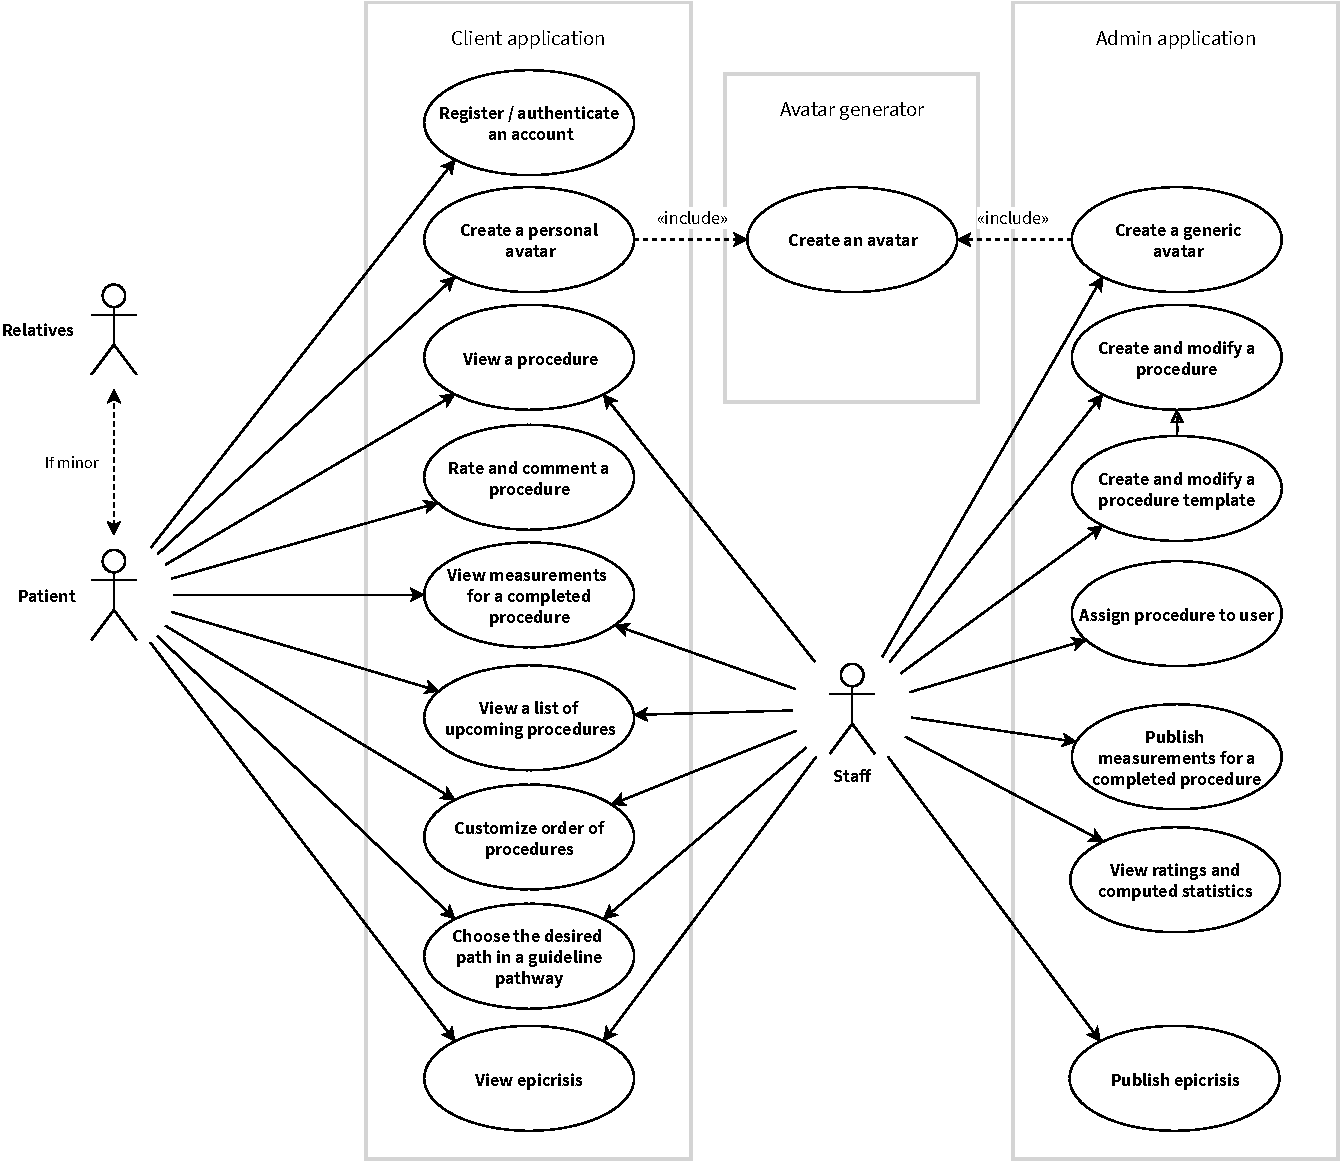
\includegraphics[width=1\textwidth]{use-cases-implementation.pdf}
    \caption{Extended use case diagram}
    \label{fig:usecases2}
\end{figure}

A revised and more detailed domain model is shown in \autoref{fig:domainmodel2}.

\begin{figure}
    \centering
    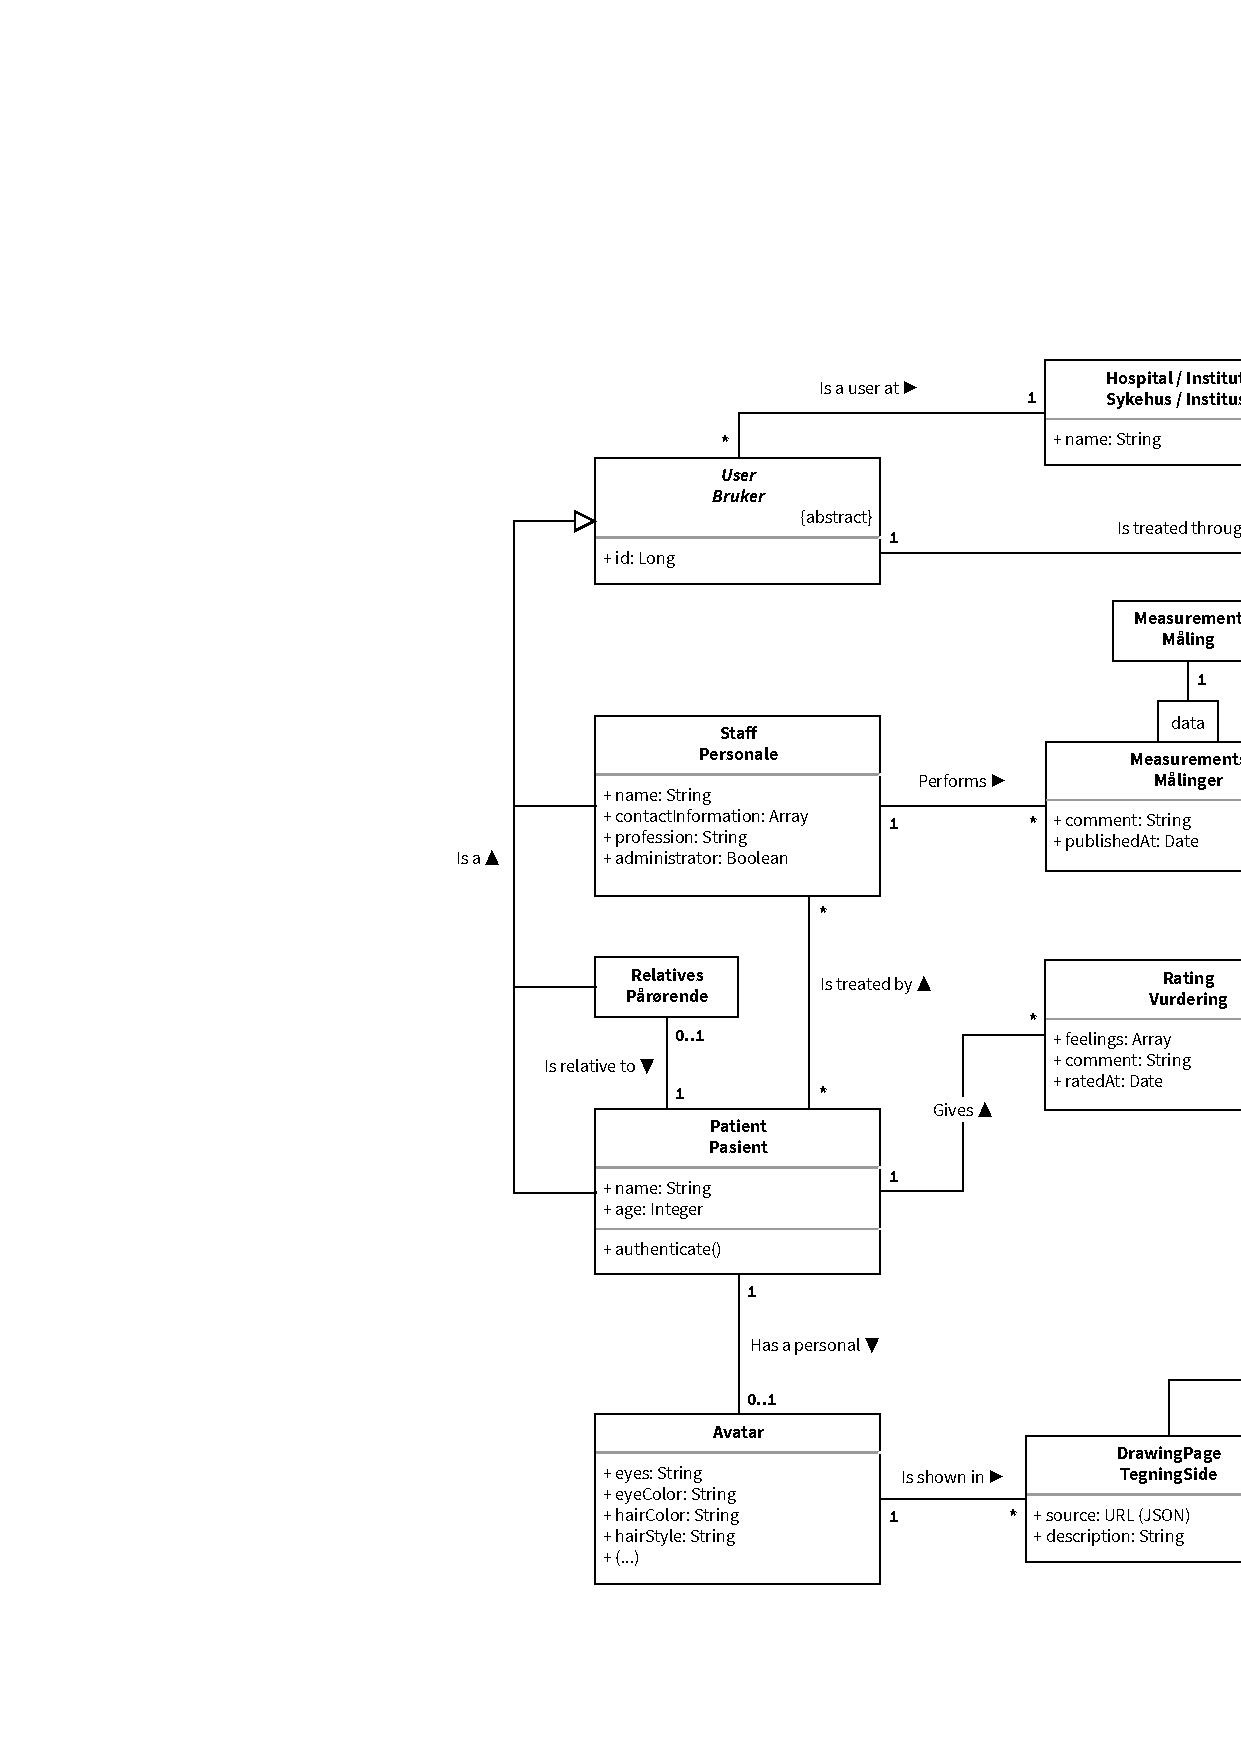
\includegraphics[width=1\textwidth]{domain-model-implementation.pdf}
    \caption{Extended domain model}
    \label{fig:domainmodel2}
\end{figure}

\section{Architecture}

\subsection{Backend}

\subsection{Frontend}

\section{Integration with existing systems}

When viewing this application together with existing systems, it . The application can be used in many steps of a particular guideline pathway. The application's flow of information can be seen in light of a guideline pathway, and the model seen in figure \ref{fig:applicationmodel} takes the guideline pathway of mental disorders for children and youth \autocite{helsedirektoratet2019} as an example.

\begin{figure}
    \centering
    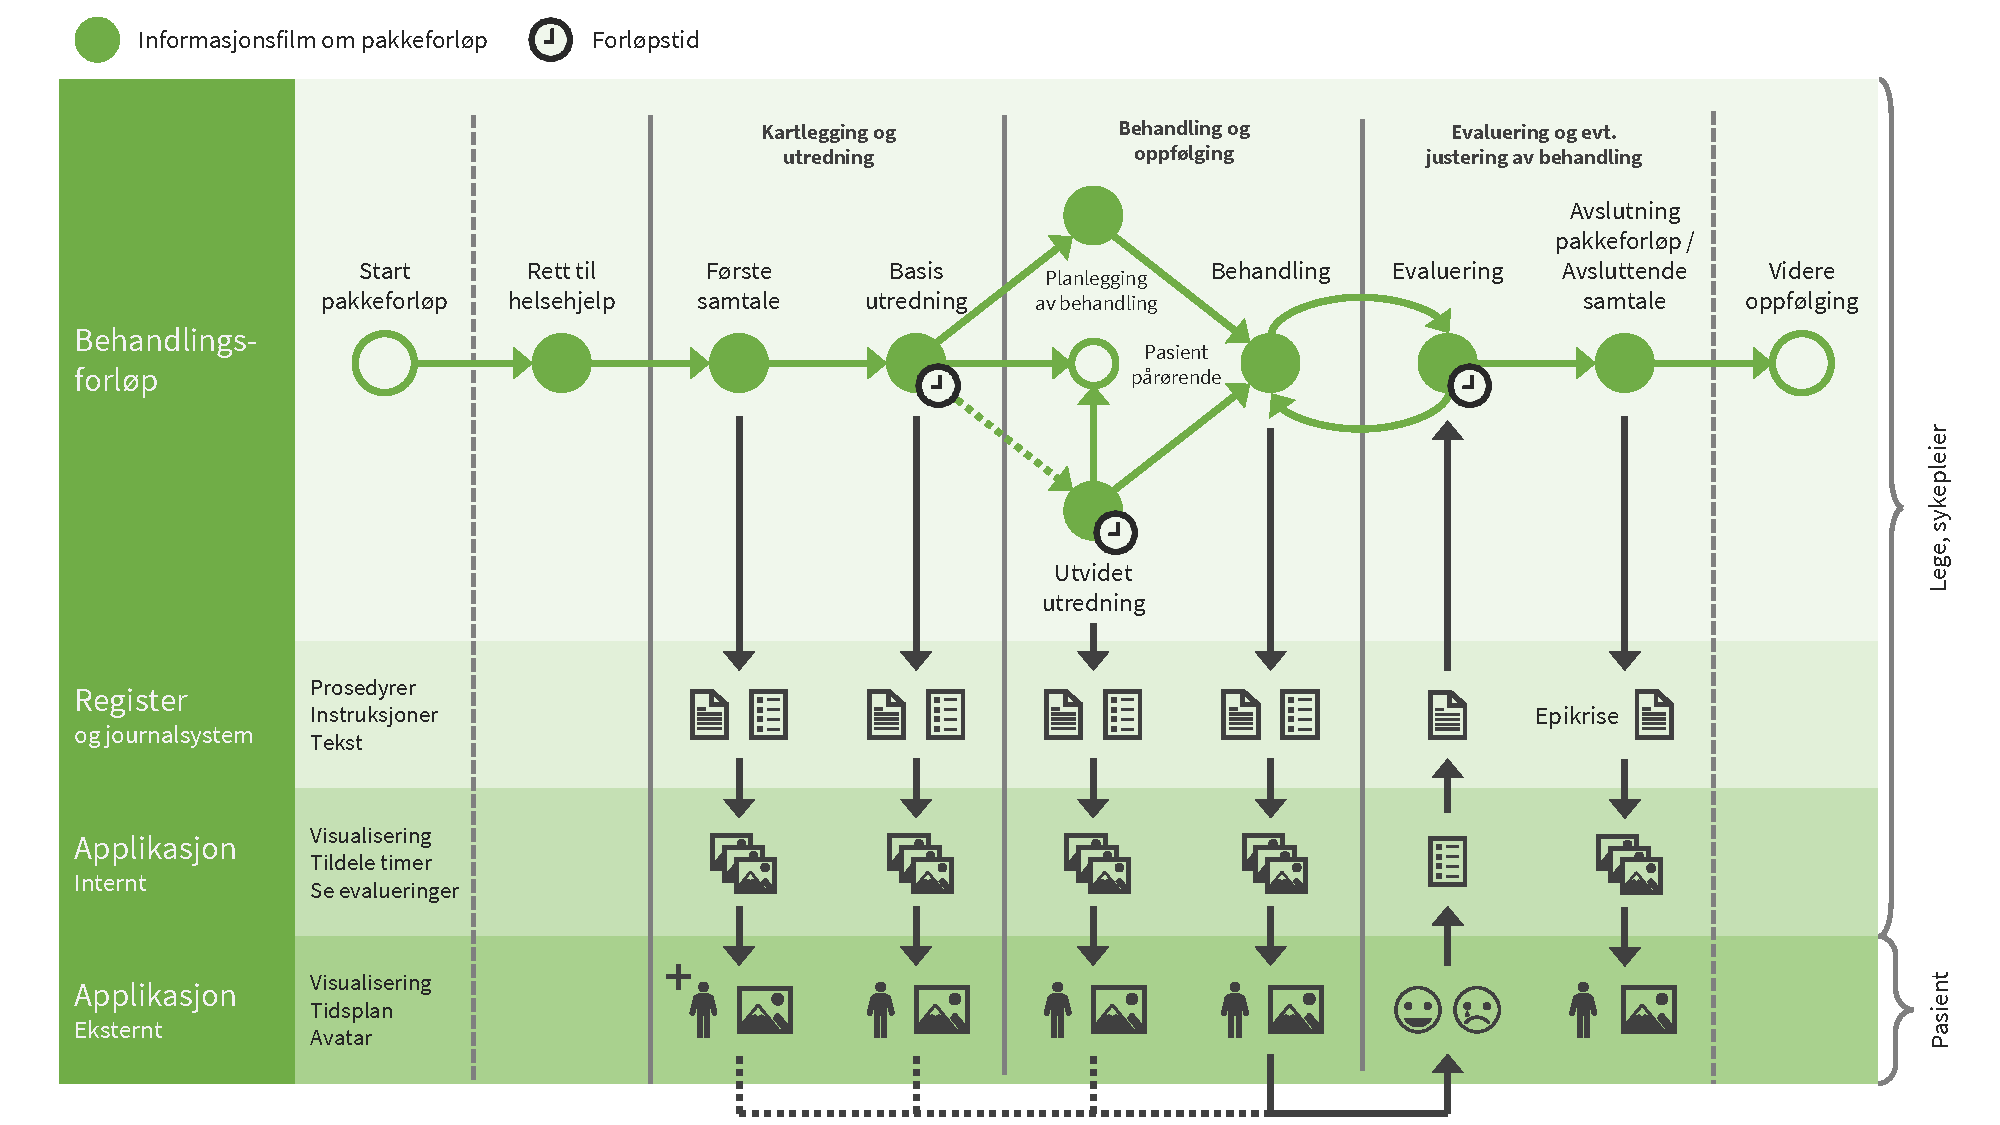
\includegraphics[width=1\textwidth]{application-model.pdf}
    \caption{Application model as illustrated through a guideline pathway}
    \label{fig:applicationmodel}
\end{figure}

This application is intended to be used together with the avatar generation system from E-LAN described in \cref{sec:relatedwork}.
The software seems to run on Windows with support for a web client, and outputs two-dimensional portrait pictures.

\section{Anticipated challenges and feasibility}
\label{sec:anticipatedchallenges}

The development tools chosen for an application should support the functionality of the application. The following subsections illustrate a few scenarios which the chosen development tools should support.

\subsection{Personalised avatars}

The avatar generation system created for E-LAN (from \ref{sec:relatedwork}) can be used together with the application. This enables the user to view their avatar in procedures like they were participating themselves. A challenge lies in associating an avatar to each user while making it easy to modify it when needed. The system is based on a graphical user interface and does not present an API; it is very much a black box where the result is an exported PNG file.

\subsection{Realistic avatar projections}

The system outputs two-dimensional portrait images only, with the face and chest facing forward. The images are also limited to the top part of the body, leaving the lower body out. Concerns were raised about whether these images would look realistic in certain settings. For example, using a single 2D image, a person laying in the bed would look awkward unless viewed from above the bed. To deal with this, there are several approaches as seen in table \ref{tab:projecting-avatar}.

% Figure showing avatar

% Figure with 4 images showing the different projections?

\begin{table}
    \centering
    \begin{tabu}{L[0.75] l L[0.5] l L}
        \textbf{} & \textbf{Realism} & \textbf{Processing \newline power} & \textbf{Ease of use} & \textbf{Additional \newline requirements} \\ \hline
        \textbf{2D images} & Lowest & Lowest & Highest & None \\ \tabucline[hdottedline]{-}
        \textbf{2D image sets with various poses} & High & Low & High & Extra image sets \\ \tabucline[hdottedline]{-}
        \textbf{2D images rotated in 3D} & Low & High & Low & Software framework which supports 3D rotations \\ \tabucline[hdottedline]{-}
        \textbf{3D models} & Highest & Highest & Lowest & New 3D models; a 3D rendering engine; software framework which supports 3D rotations \\ \hline
    \end{tabu}
    \caption{Different ways to project an avatar on a screen}
    \label{tab:projecting-avatar}
\end{table}

It is shown that 2D images can be rotated in 3D pretty realistically. \textcite{rivers2010} carried out a project which showed that it is possible to view a figure from any angle when given three 2D projections of it.

Though, an alternative is to simply use such avatars in 2D-space. 

The IACTA application shows that this can be used with similar effect as a 3D-application \autocite{stalberg2018}.

\subsection{Visual art and template designs}

This brings us to the next challenge. (...)

\subsection{Connections between client and administrator applications}

(...)

\subsection{Integrations towards current healthcare systems}

(...)

\subsection{Security concerns}

(...)

\subsection{Service workers and offline content}

(...)

% Experimental technology
% Not-so-easy with web projects

\subsection{Scaling}

(...)

\subsection{Costs}

(...)

\section{Handoff}

The scope of this project involves minimal integration with existing healthcare and journal systems at the Children and Youth Clinic and Haukeland University Hospital. Given that Helse Vest IKT monitors most of said systems, it would be sensible to develop an application that can be adapted, or even be developed further on, by them. It was pointed out that the developers of the avatar generation system used well-established web technologies such as HTML, CSS and JavaScript to develop it, and that similar technologies were preferred for the new application. This led to a new direction in choosing the most suitable software tools.

Attached to this thesis are Figma project files for the client and administrator applications. The former is interactive and the one used in this project's evaluation. % and source code for an incomplete software prototype using React and create-react-app.

(...)
